\documentclass[12pt,a4paper]{article}

% Margins.
\setlength{\oddsidemargin}{0in}
\setlength{\evensidemargin}{0in}
\setlength{\headheight}{12pt}
\setlength{\headsep}{42pt}
\setlength{\topmargin}{-60pt}
\setlength{\textwidth}{6.5in}
\setlength{\textheight}{10in}
\pagestyle{empty}

\usepackage{amsmath}
\usepackage{float}
\usepackage{graphicx}
\usepackage[hyphens]{url}
\usepackage[hidelinks]{hyperref}	% Clickable links to figures, references and urls.
\usepackage{lastpage}
\usepackage{array}
\usepackage{afterpage}

% Drawing.
\usepackage{pgf}
\usepackage{tikz}

% Listings for formatting code.
\usepackage{listings}
\usepackage{textcomp}
% General options.
\lstset{breaklines=true, basicstyle=\footnotesize\ttfamily, tabsize=4, numbers=none, stepnumber=1, frame=none, showstringspaces=false, upquote=true}
% C++ specific high-lighting. Comments are 50/50 shades of green/black and strings coloured with 60/40 red/black mixture.
\lstset{language=[ISO]C++, commentstyle=\color{green!50!black}, keywordstyle=\color{blue}, stringstyle=\color{red!60!black}}

% Marks of each question.
\def\QOne{20}
\def\Qtwo{20}
\def\Qthree{20}
\def\Qfour{20}
\def\Qfive{20}
\def\Qsix{10}
\def\Qseven{10}
\def\Qeight{10}
\def\Qnine{10}
\def\Qten{10}
\def\TotalMarks{100}

\newcommand\emptypage[1]
{
	\newpage
	\thispagestyle{empty}
	\mbox{}
}
    
\begin{document}
\begin{minipage}{0.55\textwidth}
{\LARGE \textbf{Programming for Engineers -- II}}\\[0.15cm]
{\normalsize \textbf{Spring 2014 Semester}}\\
{\Large \textbf{Final Exam}}\\
{\normalsize \textbf{Friday, May 16, 2014}}\\[0.30cm]
{\Large \textbf{Total Time: 180 minutes}}\\[0.15cm]
{\Large \textbf{Total Marks: 100}}\\
\textbf{Course Instructor:}\\
Attique Dawood\\
\end{minipage}
\begin{minipage}{0.4\textwidth}
\textbf{Serial} \hrulefill \\[0.25cm]
\textbf{Name} \hrulefill\\[0.25cm]
\textbf{Section} \rule{1cm}{0.2mm} \textbf{Roll No:} \hrulefill\\[0.25cm]
\textbf{Signature:} \hrulefill\\[0.25cm]
\rule{6.6cm}{0.2mm}\\
\textbf{Signature of Invigilator}\\[0.25cm]
\end{minipage}
\begin{table}[H]
\begin{center}
\vspace{0.3cm}
	{\large \begin{tabular}{!{\vrule width 1pt}c!{\vrule width 1pt}c!{\vrule width 1pt}c!{\vrule width 1pt}c!{\vrule width 1pt}c!{\vrule width 1pt}c!{\vrule width 1pt}c!{\vrule width 1pt}}
	\noalign{\hrule height 1pt}
		\rule{0pt}{2.6ex} Question & \textbf{1} & \textbf{2} & \textbf{3} & \textbf{4} & \textbf{5} & \textbf{Total}\\
		\noalign{\hrule height 1pt}
		Total Marks \rule{0pt}{2.6ex} & \QOne & \Qtwo & \Qthree & \Qfour & \Qfive & \TotalMarks\\
		\noalign{\hrule height 1pt}
		Marks Obtained \rule{0pt}{2.6ex} & & & & & &\\
	\noalign{\hrule height 1pt}
	\end{tabular}}
\end{center}
\end{table}
\noindent \textbf{You are advised to READ these notes:}
\begin{enumerate}
\item \textbf{Attempt on the Question Paper. \underline{NO EXTRA SHEET} will be provided/accepted. No
additional sheet will be provided for rough work. Use the back of the page where
provided space is not sufficient.}
\item After asked to commence the exam, please verify that you have \textbf{\pageref{LastPage} different
printed pages} including this title page.
\item There are 5 questions. Attempt all of them. It is advisable to go through the paper once
before starting with the first question.
\item Exam is closed books, closed notes. Please see that the area in your threshold is clean.
You will be charged for any material which can be classified as \textbf{`helping in the paper'}
found near you.
\item All distances and coordinates are in meters.
\item \textbf{Calculator sharing is strictly prohibited.}
\item Students who attempt the paper with lead pencils lose the right to get them rechecked.
\item \textbf{The invigilator present is not supposed to answer any questions. No one may come
to your room for corrections and you are not supposed to request to call anyone.
Make assumptions wherever required and clearly mark them.}
\end{enumerate}
\newpage
\noindent\textbf{Question 1: Complex Matrix\hfill \QOne~marks}\\
Write the class definitions of \verb|Complex| and \verb|Matrix| classes from assignment 03 related to operator overloading. Only class definition and prototypes of functions is required.
\begin{lstlisting}
// Complex.h
#include<iostream>
using namespace std;
class Complex
{
private:
	float real;
	float img;
public:
	friend istream& operator>>(istream&,Complex&);
	friend ostream& operator<<(ostream&,Complex);

	Complex operator+(Complex&);
	Complex operator-(Complex&);
	Complex operator*(Complex&);
	Complex operator/(Complex&);

	bool operator==(Complex&);
	bool operator!=(Complex&);
	bool operator>=(Complex&);
	bool operator<=(Complex&);
	bool operator>(Complex&);
	bool operator<(Complex&);
};
\end{lstlisting}
\begin{lstlisting}
// Matrix.h
#include "Complex.h"
class Matrix
{
private:
	int Rows;
	int Cols;
	Complex data[100][100];
public:
	Matrix(const Matrix&);

	friend istream& operator>>(istream&,Matrix&);
	friend ostream& operator<<(ostream&,Matrix);

	Matrix operator=(Matrix);
	Matrix operator+(Matrix&);
	Matrix operator-(Matrix&);
	Matrix operator*(Matrix&);

	bool operator==(Matrix&);
	bool operator!=(Matrix&);
	bool operator>=(Matrix&);
	bool operator<=(Matrix&);
	bool operator>(Matrix&);
	bool operator<(Matrix&);
};
\end{lstlisting}
\newpage
\noindent\textbf{Question 2: Object--Oriented Design\hfill \Qtwo~marks}\\
Create UML design of a classroom. First make a list of different classes with their attributes and functions and then create a flow--chart showing relationship between them.
\begin{figure}[H]
\centering
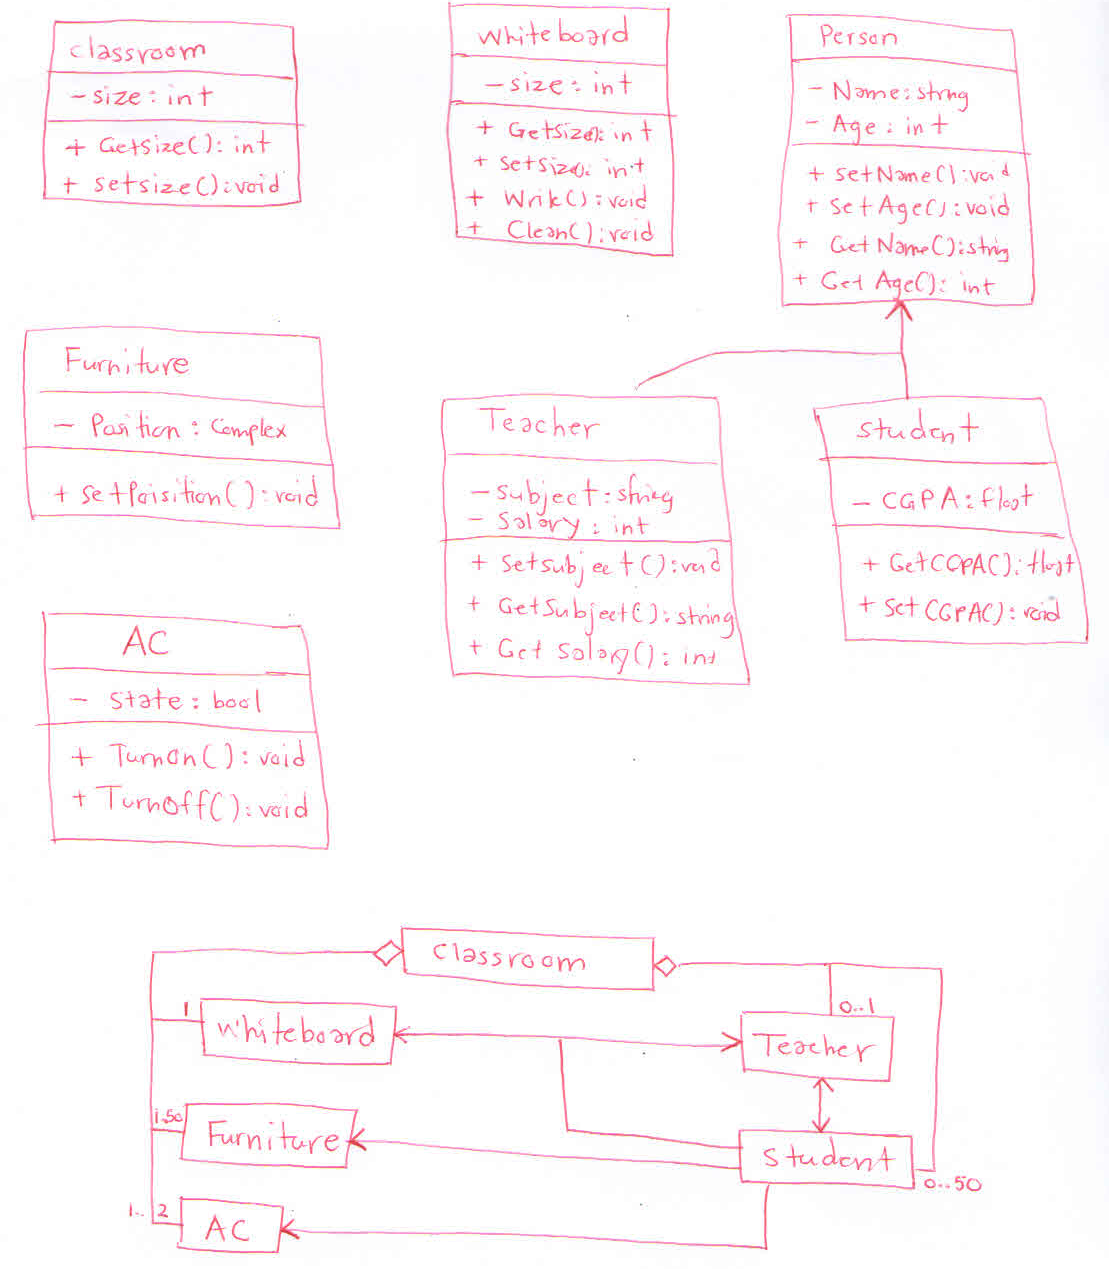
\includegraphics[scale=0.6]{UMLDiagram.png}
\end{figure}
\newpage
\noindent \textbf{Question 3: Linked List\hfill \Qthree~marks}\\
Implement a singly--linked list. Implement following functions:
\begin{itemize}
\item[a.] Add node.
\item[b.] Display all nodes.
\item[c.] Search node.
\item[d.] Array subscript operator.
\end{itemize}
\begin{lstlisting}
#include <iostream>
using namespace std;
// Node
class Node
{
public:
	int Data;
	Node* Next;
};
// Linked list class.
class LinkedList
{
private:
	Node* First;
	int Count;
public:
	// Constructor.
	LinkedList(): First(NULL), Count(0)
	{
	}
	// Adds a node at the end of linked list.
	void AddNode(int pData)
	{
		// If creating first node we need to change first pointer.
		if (First == NULL)
		{
			Node* NewNode;
			NewNode = new Node;
			NewNode->Data = pData;
			NewNode->Next = NULL;
			First = NewNode;
			Count++;
		}
		// We need to traverse the whole list to get to last node.
		else
		{
			// Find last node.
			Node* temp;
			temp = First;
			while (temp->Next != NULL)
				temp = temp->Next;
			// temp now points to last node.
			Node* NewNode;
			NewNode = new Node;
			temp->Next = NewNode;
			NewNode->Data = pData;
			NewNode->Next = NULL;
			Count++;
		}
	}
	// Displays all entries in linked list.
	void Display()
	{
		Node* temp;
		temp = First;
		while(temp != NULL)
		{
			cout << "Data = " << temp->Data << endl;
			temp = temp->Next;
		}
	}
	// Search a data value.
	int Search(int Key)
	{
		Node* temp;
		temp = First;
		while(temp != NULL)
		{
			if (temp->Data == Key)
				return 0;

			temp = temp->Next;
		}
		return -1; // If we ever get here then search was unsuccessful.
	}
	// Subscript operator.
	int& operator[](int Index)
	{
		// Checking index bounds.
		if (Index < 0 || Index >= Count)
		{
			cout << "Index out of bounds. Exiting..." << endl;
			exit(-1);
		}
		else
		{
			// Move temp pointer to point to node at desired index.
			Node* temp = First;
			for (int i=0; i<Index; i++)
				temp = temp->Next;

			return temp->Data;
		}
	}
};
\end{lstlisting}
\newpage
\noindent\textbf{Question 4: File Handling and STL \hfill \Qfour~marks}\\
A binary file \verb|Data.bin| contains some data. The data is of a table containing only integer entries. The table has a fixed number of columns, i.e. 5, but variable rows. The data is stored row--wise in the file just like a matrix. Write code to
\begin{itemize}
\item[a.] Determine the file size and number of rows.
\item[b.] Create a \verb|rows|$\times$\verb|cols| 2D \verb|vector| of \verb|int| type.
\item[c.] Read the file data into \verb|vector|.
\item[d.] Display data in the form of a table/matrix.
\end{itemize}
\begin{lstlisting}
#include <iostream>
#include <fstream>
#include <cstdlib>
#include <vector>
using namespace std;
int main()
{
	fstream File;
	File.open("Data.bin", ios::in);

	// 1. Get file size.
	File.seekg(0, ios::end); // Move get pointer to end of file.
	int FileSize = (int)File.tellg();

	// 2. Creating 2D vector.
	int Cols = 5;
	int Rows = FileSize/sizeof(int)/Cols;
	vector< vector<int> > Vector2D(Rows, vector<int>(Cols, 0));

	// 3. Reading File.
	File.seekg(0); // Reset get pointer.
	for (int i=0; i<Rows; i++)
		for (int j=0; j<Cols; j++)
			File.read((char*)&Vector2D[i][j], sizeof(int));
	File.close();

	// 4. Displaying data.
	for (int i=0; i<Rows; i++)
	{
		cout << "Row " << i << ": ";
		for (int j=0; j<Cols; j++)
			cout << Vector2D[i][j] << "\t";
		cout << endl;
	}
	return 0;
}
\end{lstlisting}
\newpage
\noindent\textbf{Question 5: Network Programming\hfill \Qfive~marks}\\
You are employed to implement a Supercomputer that can add complex numbers. The Supercomputer is basically a UDP Server running on your LAN with IP \verb|192.168.1.99| and port \verb|5601|. The UDP Client will send two complex numbers to Server. The Server will return the resultant complex number back to Client. You need to write the code in \verb|main()| for both Server and Client. It is easier to transfer a complex structure rather than transfer real and imaginary parts separately.\\
\textbf{Hint:} To send a variable use \verb|SendTo((void*)&Var, sizeof(Var), Address, Port);|
\begin{lstlisting}
// Client code.
#include <Client.h>
#include <iostream>
using namespace std;
class Complex
{
public:
	int real;
	int img;
};
int main()
{
	// Create Client object.
	Client ClientObj(UDPSOCKET);

	ClientObj.CreateSocket(UDPSOCKET);
	ClientObj.InitialiseAddress(6001);
	ClientObj.Bind();

	//char ServerAddress[] = "127.0.0.1"; // local test.
	char ServerAddress[] = "192.168.1.99";
	int ServerPort = 5601;

	Complex C1, C2, Result;
	C1.real = 1;
	C1.img = 2;
	C2.real = 3;
	C2.img = 4;

	ClientObj.SendTo((void*)&C1, sizeof(C1), ServerAddress, ServerPort);
	ClientObj.SendTo((void*)&C2, sizeof(C2), ServerAddress, ServerPort);
	ClientObj.RecvFrom((void*)&Result, sizeof(Result));
	cout << "Result: " << Result.real << "+j" << Result.img << endl;
	ClientObj.CloseClientSocket();

	return 0;
}
\end{lstlisting}
\begin{lstlisting}
// Server code.
#include <Server.h>
#include <cstring>
#include <iostream>
using namespace std;
class Complex
{
public:
	int real;
	int img;
};
int main()
{
	// Create Server object.
	Server ServerObj(UDPSOCKET, 5601);

	ServerObj.CreateSocket(UDPSOCKET);
	ServerObj.InitialiseAddress(5601);
	ServerObj.Bind();

	Complex C1, C2, Result;
	ServerObj.RecvFrom((void*)&C1, sizeof(C1));
	ServerObj.RecvFrom((void*)&C2, sizeof(C2));
	Result.real = C1.real + C2.real;
	Result.img = C1.img + C2.img;
	ServerObj.SendTo((void*)&Result, sizeof(Result)); // Reply to address/port on latest received packet.
	ServerObj.CloseServerSocket();

	return 0;
}
\end{lstlisting}
\end{document}